% \RequirePackage[l2tabu, orthodox]{nag}
%% Checks for obsolete LaTeX packages and outdated commands. 
%% Does nothing as long as your syntax is right.

\documentclass[12pt]{amsart}




% Document class possibilities:
%   amsart, article, book, beamer, report, letter
% Options:
%   letterpaper, a4paper,11pt,oneside, twoside, draft, twocolumn, landscape

%% For beamer class, see my beamer template.

%% ========== Options to Toggle When Compiling ==============
%\usepackage{syntonly}
%\syntaxonly


%%%%%%% Show Keys %%%%%%%%%%%%%%%%%%%
%\usepackage[notcite]{showkeys} 

%%%%%%%%%%%%%%%%%%%%%%%%%%%%%%%%%%

%% Show tags and labels.
% %\usepackage{layout}            %% Show variable values controlling page layout.
%\allowdisplaybreaks[1]         %% Allow multiline displays to split.
%\nobibliography     %% Use proper citations, but do not generate bibliography.

%% ========== Select *.tex file encoding and language ==============
%\usepackage[language]{babel} %% Takes care of all language requirements.

%\usepackage[latin1]{inputenc}  %% Use with PuTTY or TeXMaker
%\usepackage[utf8]{inputenc}  %% Use on most OS's, such as Ubuntu.

%% ============== Page Styles ==============
 \usepackage{fancyhdr}
% \pagestyle{fancy}
% \pagestyle{empty}

%% ============== Page Layout ==============
%% Allow extra space at the bottom of pages.
% \raggedbottom     

%% Use smaller margins.
%\usepackage{fullpage}

%%Control page number placement.  \thepage is the current page number.
% \renewcommand{\headrulewidth}{0pt}
% \lhead{}
% \chead{}
% \rhead{}
% \lfoot{}
% \cfoot{\thepage}
% \rfoot{}

\usepackage[margin=1in]{geometry}  %% Can adjust the margins of individual pages
\usepackage{setspace}
\usepackage{caption}
%% Use it like this:
%% \newgeometry{left=3cm,bottom=0.1cm}
%%     ... Lines that require margins adjusted ...
%% \restoregeometry

%% ============== Math Packages ==============
\usepackage{amsmath}
\usepackage{amsfonts}
\usepackage{amssymb}
\usepackage{amsthm}
\usepackage{mathtools} % An improvement of amsmath
\usepackage{latexsym}

%% ============ Typesetting add-ons ============
%\usepackage{siunitx} %Support for SI units, \num, \SI, etc.

%% ============== Single-Use Packages ==============
\usepackage{enumerate}
\usepackage{cancel}
\usepackage{cases}
\usepackage{empheq}
\usepackage{multicol}

%% ============== Graphics Packages ==============
\usepackage{graphicx} %% Conflicts with pdflatex.
%\usepackage{graphics} %% Conflicts with eps files.
%\usepackage{epsfig} Allows eps files (?)

\usepackage{wrapfig}

%% Note: For using .eps graphics, use the graphicx package,
%% and in the document use, for example:
%% \begin{figure}
%%  \includegraphics[scale=0.5]{my_picture.eps}
%% \end{figure}

%% Prevent figures from appearing on a page by themselves:
%\renewcommand{\topfraction}{0.85}
%\renewcommand{\textfraction}{0.1}
%\renewcommand{\floatpagefraction}{0.75}

%% Force floats to always appear after their definition: 
%\usepackage{flafter}

%% ============== tikZ and PGF packages ==============
%\usepackage{ltxtable,tabularx,tabulary}
 
% \usepackage{tikz}
% \usepackage{pgf}
% \usepackage{pgfplots} %% Requires pgf 2.0 or later.
% % \usetikzlibrary{arrows, automata, backgrounds, calendar, 
% % chains,matrix, mindmap, patterns, petri, shadows, 
% % shapes.geometric,shapes.misc,
% % spy, trees}
% \pgfplotsset{compat=1.9} % Fixes some backwards compatibility warnings
% \usetikzlibrary{arrows}

%% ============== Colors ==============
%% Warning: These are often a source of conflicts during compilation.
\usepackage{color}
\newcommand{\blue}[1]{{\color{blue} #1}}
\newcommand{\red}[1]{{\color{red} #1}}

%% ============== Notes ==============
\usepackage[color=white,linecolor=black]{todonotes}
% \usepackage[backgroundcolor=gray!30,linecolor=black]{todonotes}
% \usepackage[disable]{todonotes}
%\listoftodos, \todo[noline]{}, \todo[inline]{}, \todo{}, \missingfigure{}
% \todo]{}
   
%% ============== Fonts ==============
%\usepackage{bbm}  %% Non-Vanilla: Not include in many LaTeX distributions.
\usepackage{mathrsfs}
\usepackage{fontenc} %T1 font encoding
\usepackage{inputenc} %UTF-8 support
%\usepackage{babel} %Language specific commands, shortcuts, hyphenation.

\usepackage{verbatim}

%% Microtype improves spacing.  Load after fonts.
% \usepackage{microtype}

%% ============== Theorem Styles ==============
%% Note: newtheorem* prevents numbering.

\theoremstyle{plain}
\newtheorem{theorem}{Theorem}[section]
\newtheorem{proposition}[theorem]{Proposition}
\newtheorem{lemma}[theorem]{Lemma}
\newtheorem{corollary}[theorem]{Corollary}
\newtheorem*{claim}{Claim}

\theoremstyle{definition}
\newtheorem{definition}[theorem]{Definition}
\newtheorem{example}[theorem]{Example}
\newtheorem{exercise}[theorem]{Exercise}
\newtheorem{axiom}[theorem]{Axiom}

\theoremstyle{remark}
\newtheorem{remark}[theorem]{Remark}

%% ============== References ==============
\setcounter{secnumdepth}{3} %% Used to label subsections
\numberwithin{equation}{section} %% Equation numbering control.
\numberwithin{figure}{section}   %% Figure numbering control.

\usepackage[square,comma,numbers,sort&compress]{natbib}
\usepackage[colorlinks=true, pdfborder={ 00 0}]{hyperref}
\hypersetup{urlcolor=blue, citecolor=red}
\usepackage{url}

%% Reference things as 'fig. 1', 'Lemma 7', etc.
\usepackage{cleveref}

%% Create references like 'on the following page', 'on page 23'
% \usepackage{varioref} 

% usepackage[refpages]{gloss} %% Glossary

%%%%%%%%%%%%%%%%%%%%% MACROS %%%%%%%%%%%%%%%%%%%%%

% ============================== Vectors ==============================
\newcommand{\vect}[1]{\mathbf{#1}}
\newcommand{\bi}{\vect{i}}
\newcommand{\bj}{\vect{j}}
\newcommand{\bk}{\vect{k}}

\newcommand{\bn}{\vect{n}}

\newcommand{\bu}{\vect{u}}
\newcommand{\bv}{\vect{v}}
\newcommand{\bw}{\vect{w}}
\newcommand{\boldm}{\vect{m}}
\newcommand{\bx}{\vect{x}}
\newcommand{\by}{\vect{y}}
\newcommand{\bz}{\vect{z}}

\newcommand{\be}{\vect{e}}
\newcommand{\bg}{\vect{g}}

\newcommand{\bbf}{\vect{f}}

% ==================== Fields ==================
\newcommand{\field}[1]{\mathbb{#1}}
\newcommand{\nN}{\field{N}}
\newcommand{\nZ}{\field{Z}}
\newcommand{\nQ}{\field{Q}}
\newcommand{\nR}{\field{R}}
\newcommand{\nC}{\field{C}}
\newcommand{\nF}{\field{F}}
\newcommand{\nK}{\field{K}}

% ======================== Script Symbols  ========================
\newcommand{\sL}{\mathscr L}
\newcommand{\sH}{\mathscr H}
\newcommand{\sG}{\mathscr G}

% ====================== Caligraphic Symbols ======================
\newcommand{\cA}{\mathcal A}
\newcommand{\cB}{\mathcal B}
\newcommand{\cC}{\mathcal C}
\newcommand{\cD}{\mathcal D}
\newcommand{\cF}{\mathcal F}
\newcommand{\cH}{\mathcal H}

\newcommand{\cK}{\mathcal K}
\newcommand{\cL}{\mathcal L}

% ======================== Fraktur Symbols  ========================
% Note: Use mathrsfs package.

\newcommand{\fm}{\mathfrak m}

% ========================== Bold Symbols ==========================
\newcommand{\bvphi}{\boldsymbol{\vphi}}
\newcommand{\bPhi}{\boldsymbol{\Phi}}

% ======================== Misc. Symbols ========================
\newcommand{\nT}{\mathbb T}
\newcommand{\vphi}{\varphi}
\newcommand{\maps}{\rightarrow}
\newcommand{\Maps}{\longrightarrow}
\newcommand{\sand}{\quad\text{and}\quad}
\newcommand{\QED}{\hfill$\blacksquare$}
\newcommand{\tac}{\textasteriskcentered}
%\newcommand{\dhr}{\m\athrel{\lhook\joinrel\relbar\kern-.8ex\joinrel\lhook\joinrel\rightarrow}}

% ========================== Operations ==========================
\newcommand{\cnj}[1]{\overline{#1}}
\newcommand{\pd}[2]{\frac{\partial #1}{\partial #2}}
\newcommand{\npd}[3]{\frac{\partial^#3 #1}{\partial #2^#3}} %\npd{f}{x}{2}
\newcommand{\abs}[1]{\left\lvert#1\right\rvert}
%\newcommand\norm[1]{\left\vert\mkern-1.7mu\left\vert#1\right\vert\mkern-1.7mu\right\vert}
%\newcommand\bnorm[1]{\bigl\vert\mkern-2mu\bigl\vert#1\bigr\vert\mkern-2mu\bigr\vert}
\newcommand{\set}[1]{\left\{#1\right\}}
\newcommand{\ip}[2]{\left<#1,#2\right>}
\newcommand{\iip}[2]{\left<\left<#1,#2\right>\right>}
\newcommand{\braket}[1]{\left<#1\right>}
\newcommand{\pnt}[1]{\left(#1\right)}
\newcommand{\pair}[2]{\left(#1,#2\right)}

%Advection operators:
\newcommand{\adv}[2]{(#1 #2)}
\newcommand{\vectadv}[2]{\;#1 \otimes#2\;}

% ============ Special Macros For This Paper ==================
\newcommand{\diff}[1]{\widetilde{#1}}
\newcommand{\bud}{\diff{\bu}}
\newcommand{\ud}{\diff{u}}


% \newcommand{\weaklim}[1]{\substack{\mathrm{wk\mbox{-}lim}\\[0.1ex]#1}}
\DeclareMathOperator*{\weaklim}{wk-lim}

% ========================== Norms ==========================
\newcommand{\norm}[1]{\left\|#1\right\|}
\newcommand{\snorm}[2]{\left\|#1\right\|_{#2}}
\newcommand{\normH}[1]{|#1|}
\newcommand{\normV}[1]{\|#1\|}
\newcommand{\normLp}[2]{\|#2\|_{L^{#1}}}
\newcommand{\normHs}[2]{\|#2\|_{H^{#1}}}
\newcommand{\normLL}[3]{\|#3\|_{L^{#1}([0,T],L^{#2})}}
\newcommand{\normLH}[3]{\|#3\|_{L^{#1}([0,T],H^{#2})}}
\newcommand{\normCL}[3]{\|#3\|_{C^{#1}([0,T],L^{#2})}}
\newcommand{\normCH}[3]{\|#3\|_{C^{#1}([0,T],H^{#2})}}
%\usepackage{fancyhdr}

%% ============== Counters ==============
\newcounter{my_counter}
\setcounter{my_counter}{1} 

% ================== Title Page ========================
% Remove the author and date fields and the space associated with them
% from the definition of maketitle.
% \makeatletter
% \renewcommand{\@maketitle}{
% \newpage
%  \null
%  \vskip 2em%
%  \begin{center}%
%   {\LARGE \@title \par }%
%  \end{center}%
%  \par} \makeatother

 % ====================== Article Information ======================
\title[Data Assimilation for Reaction-Diffusion]{A Computational Study of Data Assimilation for a Reaction-Diffusion Equation}

\date{\today}

% ======================  Author Information ======================
%\author{Adam Larios}
%\address[Adam Larios]{Department of Mathematics, 
%                University of Nebraska--Lincoln,
%        Lincoln, NE 68588-0130, USA}
%\email[Adam Larios]{alarios@unl.edu}
%
\author{Collin Victor}
\address[Collin Victor]{Department of Mathematics, 
                University of Nebraska--Lincoln,
        Lincoln, NE 68588-0130, USA}
\email[Collin Victor]{collinzacharyvictor@gmail.com}
%


\keywords{}
\thanks{MSC 2010 Classification: }

\begin{document}
	\doublespacing
%==============================================================-
%\begin{abstract}
% Abstract goes here. (Don't write until we are finished.)
%\end{abstract}
\begin{titlepage}
	\begin{center}
		\vspace{3cm}\large
	A Computational Study of Data Assimilation\\ for a Reaction-Diffusion Equation\\

		\vspace{3cm}
		\normalsize
		An Undergraduate Honors Thesis\\
		Submitted in Partial fulfillment of\\
		University Honors Program Requirements\\
		University of Nebraska-Lincoln
		\vspace{3cm}
		by\\
	Collin Victor, BS\\
		Mathematics and Computer Science\\
		College of Arts and Sciences\\
\vfill
		\today\\
		\vspace{3cm}
		Faculty Mentors:\\
		Adam Larios, PhD, Mathematics\\
		\vspace*{3cm}
		
		
	\end{center}
\end{titlepage}
% =====================================================================
\section*{Abstract}\label{abstract}
% =====================================================================
This research project applied the  Azouani-Olson-Titi data assimilation algorithm \cite{AOT1,AOT2} to the 1D Chafee-Infante equation in order to investigate the potential for different grid configurations. It was discovered that for certain $\nu$ values convergence could be increased by replacing a uniform grid by a moving cluster of points. In addition to this, this study found a heuristic argument solving the inverse problem of determining the minimum length given the minimum number of nodes required for convergence. All simulations were conducted using a semi-implicit convex splitting numerical scheme \cite{Eyre} and spatial derivatives were approximated using second-order finite difference approximations. 

\pagenumbering{gobble}
\bfseries{Key Words:}
\normalfont
Data Assimilation, Chafee-Infante, Mathematics 
\newpage
\pagenumbering{arabic}

% =====================================================================
\section*{Dedication}\label{dedication}
% =====================================================================
\pagenumbering{gobble}
This research was partially supported by grant numbers... .
\todo{Official UCARE stuff goes here}
\newpage
\pagenumbering{arabic}
%\maketitle
%\begin{abstract}
%	hello
%\end{abstract}
%\maketitle
%\thispagestyle{empty}%Gets rid of page number on first page.
%============================================================
% =====================================================================
%\section{Abstract}\label{abs}
%% =====================================================================
%\noindent
%\begin{abstract}
%	hhhee
%	this is the abstract
%\end{abstract}

%\noindent
\maketitle
%\rhead{\thepage}
%\thispagestyle{plain}
% =====================================================================
\section{Introduction}\label{secInt}
% =====================================================================
\noindent
In many simulation-driven fields that involve real-world data, such as numerical prediction of weather on earth and on the sun, a central problem arises. Namely, initial data may be known at a small number of locations, such as the temperature or wind speed measured at weather stations. Without this data, evolving the system in time is highly error prone. Data assimilation is an approach that eliminates the need for complete initial data. Instead, it incorporates incoming data into simulations by penalizing deviations from the data, driving the system to the ``true'' solution.

Classical data assimilation is based on an algorithm known as Kalman Filtering. This technique and its modifications have a long history, but it still suffers from many drawback when applied to nonlinear problems, such as those in turbulent flows. In 2013 a new approach was developed, known as the Azouani-Olson-Titi (AOT) algorithm \cite{AOT1,AOT2}. The AOT algorithm incorporates the data at the level of the underlying partial differential equation. It acts as a continuous feedback-control mechanism, using incoming data to drive the simulation to the correct solution. The algorithm is given by:
\begin{align*}
\frac{d}{dt}v = F(v,t) - \mu(I_h(y)-I_h(v)), &~v(0) = 0.
\end{align*}
Here, $\mu \geq 0$ is a constant, and $I_h$ is an interpolation operator for a grid, h. y is given by the following:
\begin{align*}
\frac{d}{dt}y = F(y,t),& ~y(0) = y_0.
\end{align*}
The number of grid points in h is a very important parameter for data assimilation. If the grid has too few points, the solution will never converge, but having more points than required adds unnecessary computational complexity. In addition to this, in real world scenarios (such as weather prediction) where these grid points are marked by censors (or weather stations), minimizing the number of grid points reduces the financial cost of censor production and placement. This study examines whether we can achieve the same level of convergence using fewer points and without sacrificing numerical stability by using different grid configurations.

This study examines the potential for non-uniform sensor placement as a viable strategy for data assimilation for reaction-diffusion equations. The specific equation used in this study is the 1D Chafee-Infante equation:
\begin{align*}
u_t - \nu u_{xx} &= u - \alpha u^3\\
u(x,0) &= u_0(x)
\end{align*}
where $\alpha>0, \nu>0$ with Dirichlet boundary conditions.

Normally data assimilation uses data collected at points on a uniform grid. This study examines how the use of a moving cluster of sensors instead of a static uniform grid affects the convergence of the system to the true solution in the context of reaction-diffusion equations. By altering the placement of the nodes it is hoped that it will reduce the minimum number of grid points required for convergence to the true solution.

This study has experimentally found a bound for the number of grid points in $h$ for the uniform grid required for convergence using periodic initial data. A heuristic argument for a relationship between the size of h required for convergence and the minimum length, $\lambda$, using only data assimilation was also found. In addition to this, it was found that for certain values of $\nu$ that using a moving cluster of points does in fact require fewer grid points.

%This study uses a semi-implicit convex splitting scheme from \cite{Eyre} \todo{Add Bibliography entry} to recover both the actual solution and the simulated data assimilation solution. Simulations have two distinct phases, an initial ramp up phase allows the actual solution to transition to a stable state, after this the actual solution and the simulated AOT algorithm solution run in tandem using a some grid configuration of h points. After a set number of time-steps, the error is measured and the second phase is repeated using a binary search algorithm to determine the minimum number of grid points of h with sufficient convergence.    



% =====================================================================
\section{Preliminaries}\label{secPre}
% =====================================================================
\noindent
The Chafee-Infante equation is given by: 
\begin{align*}
u_t - \nu u_{xx} = u - \alpha u^3,\\
u(x,0) = u_0(x)
\end{align*}
where $\alpha>0, \nu>0$, and with Dirichlet boundary conditions. We solved this equation on a uniform grid of $N$ points distributed uniformly on $\left[0,1\right]$ using discrete time-steps of size $dt$. To ensure that initial data had a fully-resolved spectrum we used:
\begin{align*}
u_0 = \sum_{k=1}^{\frac{N}{4}}a_k\sin(2\pi kx)
\end{align*}
where $a_k$ is some integer. The Chafee-Infante equation is a good equation to use for this study because of its well-documented (?) features. Solutions to this equation have three distinct phases. The equation initially develops based on the initial data and reaches a mostly stable state. This stable state consists of large ``blobs'' of positive and negative activity with transition layers in between (see \cref{fig:example}). The system will then eventually decay to 0, although this behavior is not what we are trying to capture with data assimilation.
\begin{figure}
	\centering
	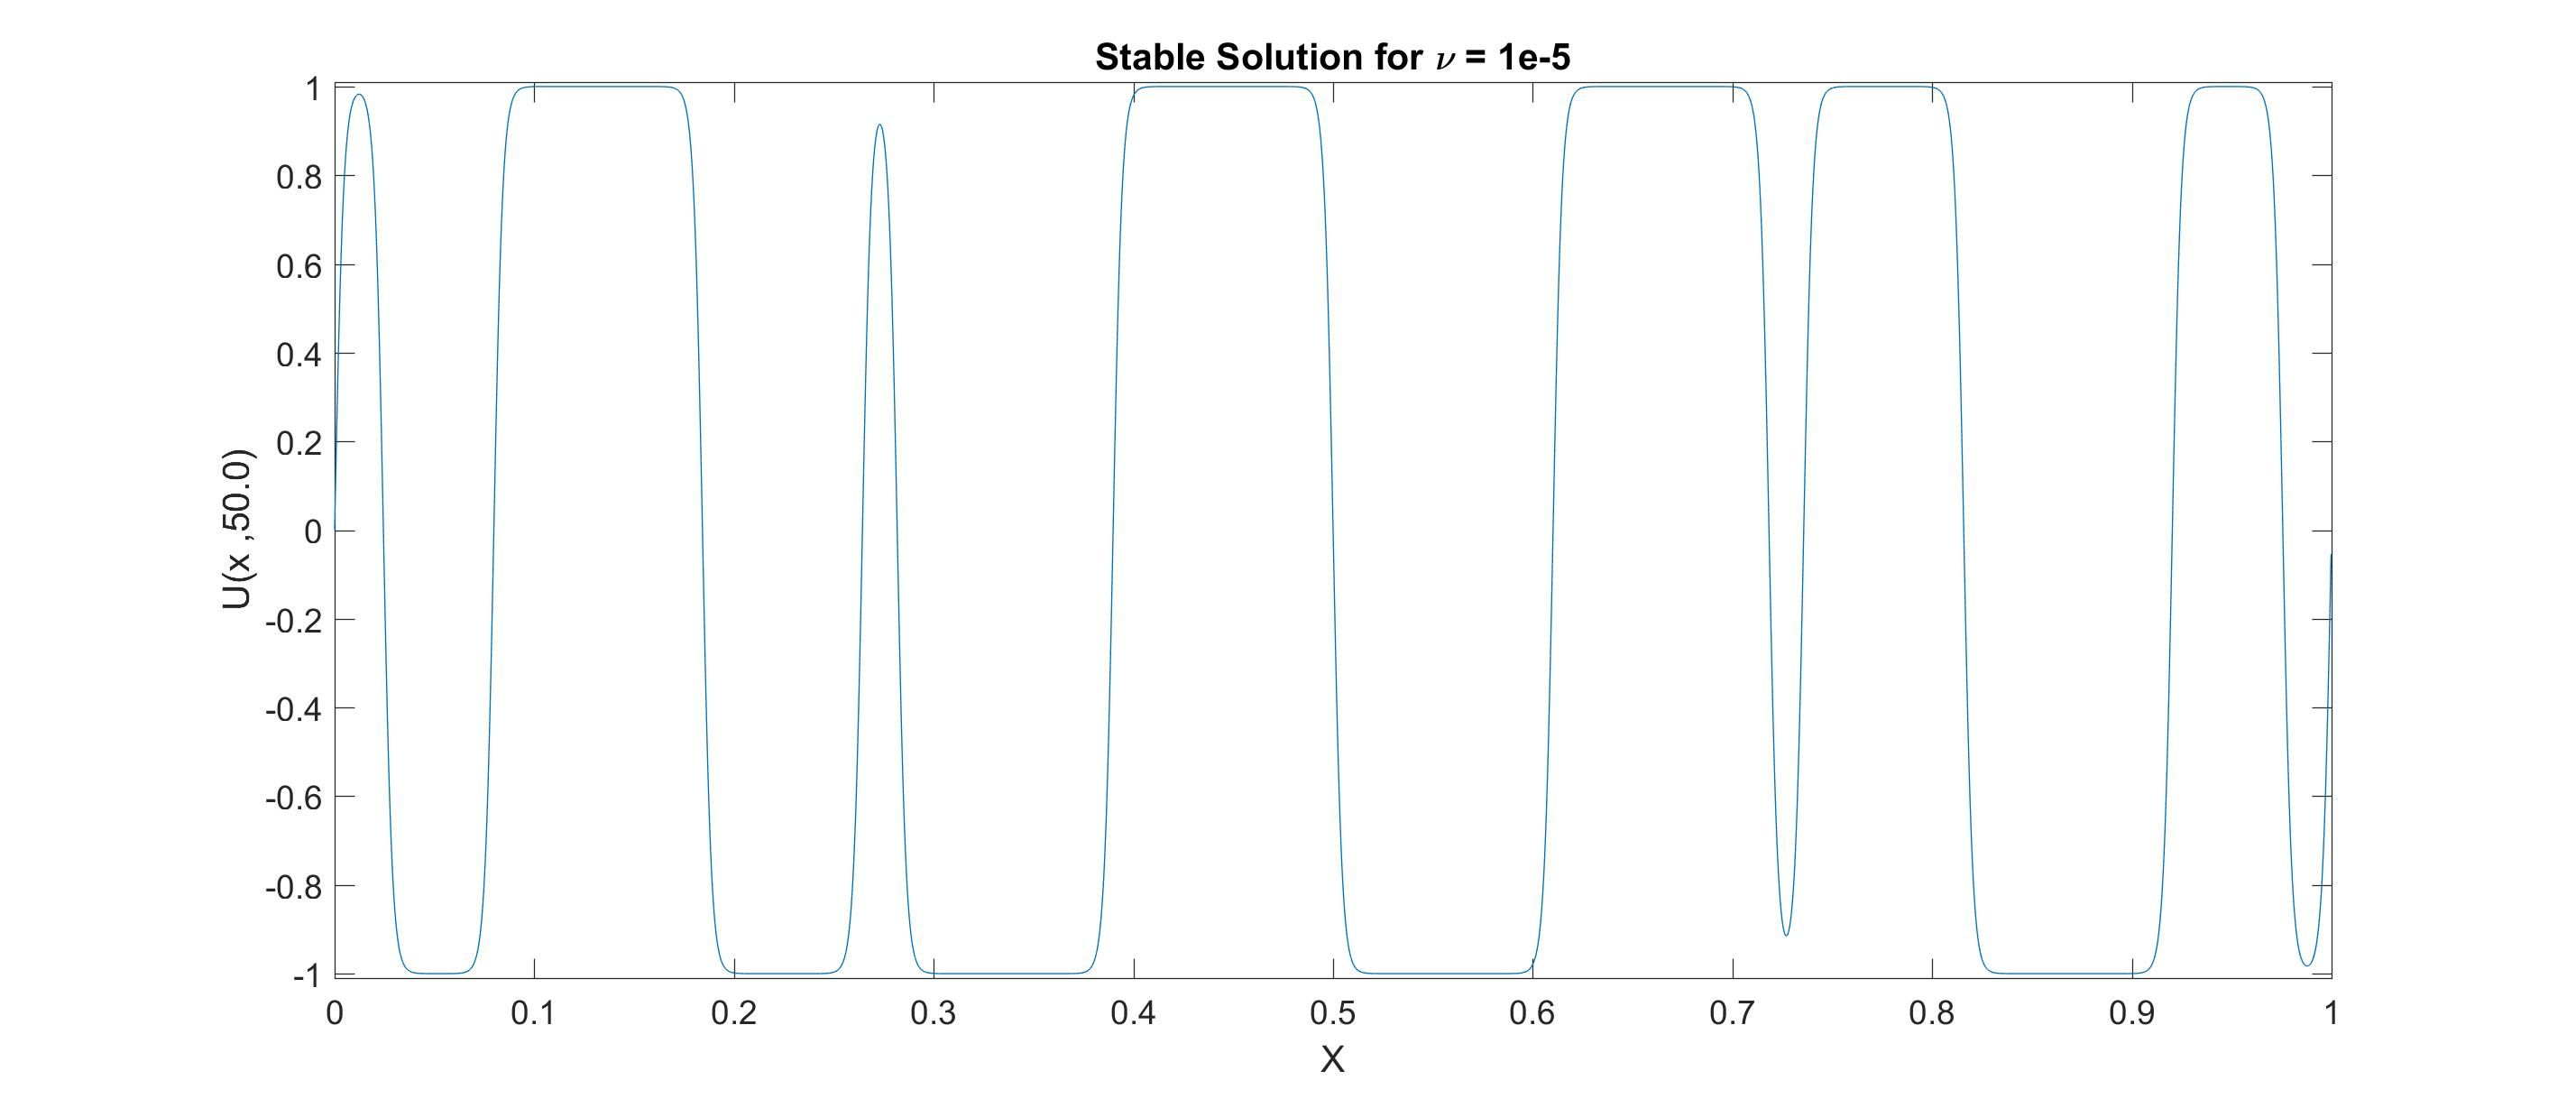
\includegraphics[scale=0.15]{Example.jpg}
	\caption{Example of a stable state solution for Chafee-Infante equation $\alpha = 1$ $\nu=1e-5$  $N = 2^{12}$}
	\label{fig:example}
%	\caption{}
\end{figure}

This study uses a semi-implicit convex splitting scheme from \cite{Eyre} \todo{Add Bibliography entry} to solve for the actual solution and the simulated data assimilation solution at every time-step. The numerical scheme is given by:
\begin{align*}
{U_k}^{n+1} - {U_k}^n = dt(\nu D_{xx} + 1+2\alpha){U_k}^{n+1} + dt(-2\alpha - \alpha {U_k}^{n^2}){{U_k}^n}
\end{align*} 
where ${U_k}^{n} = u(x_k,t_n)$ where $x_k = k dx$, $t_n = n dt$. 
%Here $x$ is discretized into $N$ points uniformly distributed on $\left[0,1\right]$ and $t$ is given in discrete time steps of size $dt$. 
$D_{xx}$ is the operator $\frac{\partial^2}{\partial x^2} $, here $\frac{\partial^2 {U_k}^{n+1}}{\partial x^2}$ is given by the second-order finite difference approximation $\frac{{U_{k-1}}^{n+1} - 2{U_{k}}^{n+1} + {U_{k+1}}^{n+1}}{dx^2} $. This results in the below system which needs to be solved at every time-step:
\begin{align*}
(1 - dt(\nu D_{xx} + 1+2\alpha)){U_k}^{n+1} =  (1+dt(-2\alpha - \alpha {U_k}^{n^2})){{U_k}^n}
\end{align*}
While this method requires us to solve a system of equations at each time-step, it is much more stable than other methods and allows us to have a much larger time-step than other methods. In addition to this, the resulting matrix is tri-diagonal, solving this system only has a time complexity of $O(n)$.

In order to apply data assimilation, the below system needs to be solved at each time-step:
\begin{align*}
(1 - dt(\nu D_{xx} + 1+2\alpha)){V_k}^{n+1} =  ({V_k}^n+dt((-2\alpha{V_k}^n - \alpha {V_k}^{n^3}) +\mu(I_h(U^n) - I_h(V^n)))
\end{align*}
Two different types of data assimilation were tested in this study, each modifying $I_h$. The first type was the standard uniform grid, $I_h(S)$ is the linear interpolation of $S$ over a uniform grid of points. The second type used a moving cluster of points which we will refer to as a sweeping probe. Data assimilation via a sweeping probe uses $I_h(S) = I_{h(t)}(S)$. Instead of uniformly distributing $m$ points, $m$ consecutive points are used at each time-step. \\
$h{(t_n)} = \left\{x_k |~ k\in [nm \text{ (mod } N),nm+m-1 \text{ (mod } N)] \subset\nZ \right\}$ Initially the first $m$ points are used, then at the next time-step, the next $m$ points are used. When the probe reaches the end of the domain, it wraps back around to the other side.  

Simulations run for this study have two distinct phases, an initial ramp up phase allows the actual solution to transition to a stable state, after this the actual solution and the simulated AOT algorithm solution run in tandem using some grid configuration of $m$ points. After a set number of time-steps, the error is measured and the second phase is repeated using a binary search algorithm to determine the minimum value of $m$ for which there is sufficient convergence. The binary search is started on the interval $\left[2,N\right]$, this interval will always contain a minimum value of $m$ as $m=N$ will always converge and the end points ($m=2$) are required nodes for the uniform grid. 
%In this section outline numerical scheme (eyre convex splitting theme) used and what I used this scheme for
%finding the minimum nodes
%Preliminaries section.  Put basic lemmas, theorems, and definitions here (i.e., the ones we are going to cite).
%
%Introduce Data Assimilation, the Chaffee-Infante equation, the Eyre convex splitting method
%https://www.math.utah.edu/~eyre/research/methods/papers.html 


% =====================================================================
\section{Parameter Estimation}\label{secNeat1Section}
% =====================================================================
\noindent
\todo{Search literature for formula for minimum length}
In this section detail how to find the minimum length $\lambda$ using nothing but data assimilation.

Through experimental trials we have found that the only requirement for consistent convergence to the true solution is to have at least one grid point in each transition layer and one in each ``blob''. It can be seen from \cref{fig:optimal} that if a transition layer does not have a grid point, the solutions may never converge. In fact by using a postereori examination of the solution, we found that if we knew where the transition layers were going to form, we can achieve convergence using this grid configuration. It seems that the most important parameter in determining the minimum number of nodes required for convergence, $M$, is the minimum length of the ``blobs'', $\lambda$. 
\begin{figure}
	\centering
	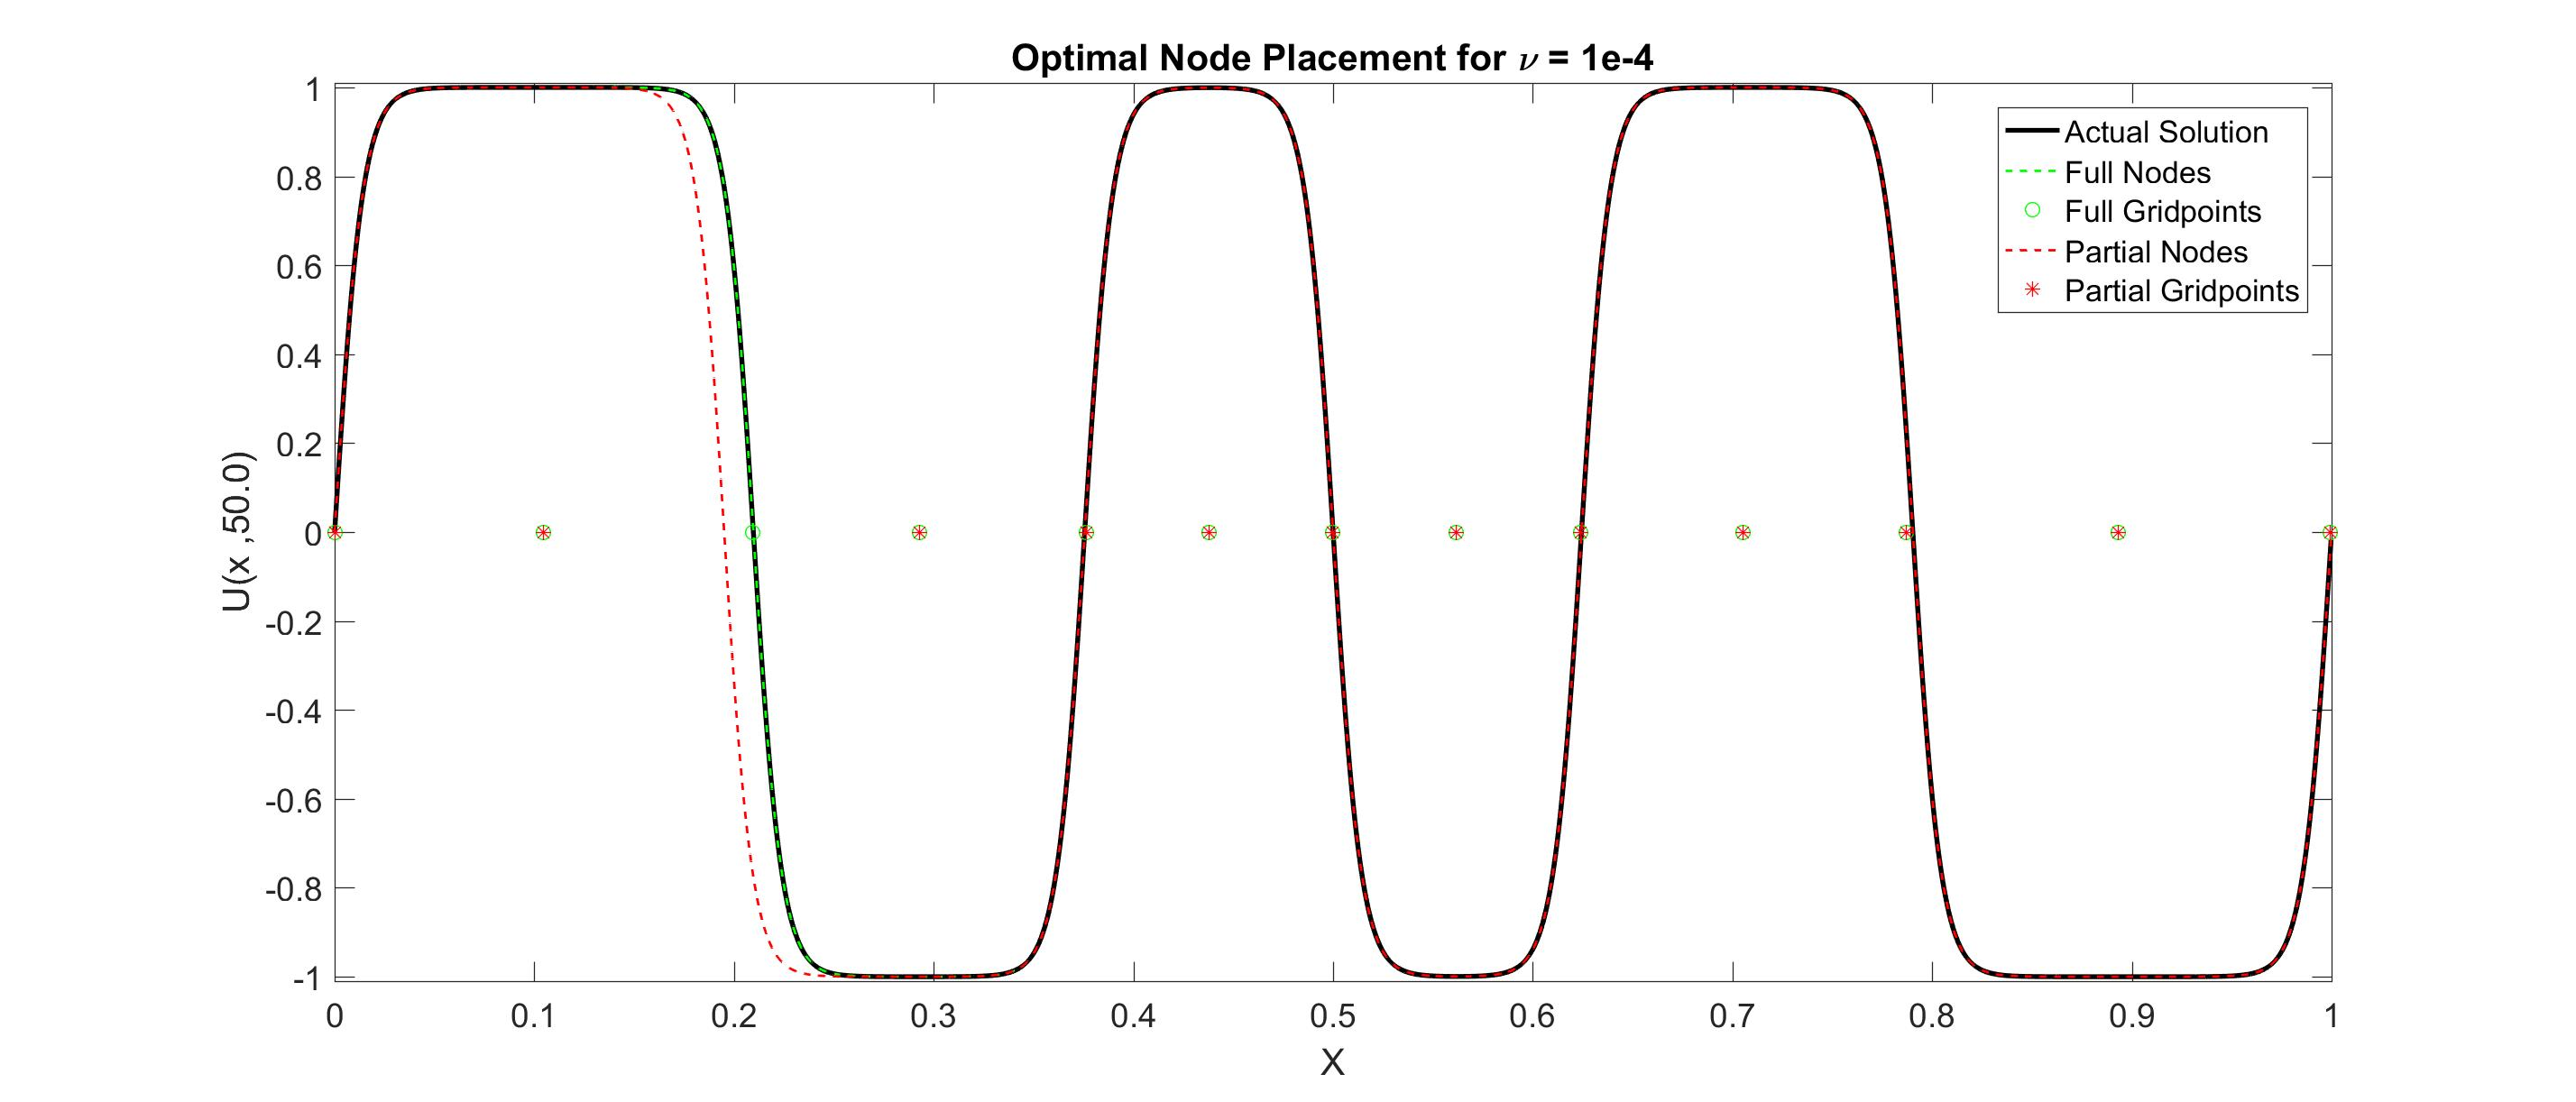
\includegraphics[scale=0.15]{Optimal.jpg}
	\caption{Data Assimilation can converge or diverge based on one grid point $\alpha = 1$ $\nu=1e-4$ $N = 2^{12}$}
	\label{fig:optimal}
	%	\caption{}
\end{figure}

From repeated experiments we discovered that $M \propto \frac{1}{4}\nu^{-\frac{1}{2}}$ in the worst-case scenario (see \ref{fig:min}). The parameter $\alpha$ affects the amplitude of the solutions, but $\nu$ is directly related to the number of ``blobs'' in the solution. The most nodes (using an optimal placement) will be required when all the ``blobs'' have the same size $\lambda$. In this case, for there being $n_b$ ``blobs'' we get $\lambda = \frac{L}{n_b} $, where $L$ is the length of the domain. We also know $M = 2n_b + 1$ or equivalently $n_b = \frac{M-1}{2}$.
\begin{align*}
\lambda & = \frac{L}{n_b}\\
&\approx\frac{2L}{M}\\
&\approx\frac{8L}{\nu^{-\frac{1}{2}}}\\
& \approx 8L\sqrt{\nu}
\end{align*}

Using only principles of data assimilation we discovered a solution for the inverse problem $\lambda \approx 8L\sqrt{\nu}$.
% =====================================================================
 \section{Sweeping Probe Data Assimilation}\label{secNeatSection}
% =====================================================================
\noindent
The main finding of this study was in the potential for sweeping data assimilation. In general it was found that for $\mu$ large enough for which the system is stable that in general far fewer nodes are required for data assimilation via a sweeping probe for sufficiently small $\nu$ (see \cref{fig:min}). Of course when $\nu$ is large it is more efficient to use a uniform grid, but there is a threshold where the methods are roughly equivalent. For $\mu =100$ this value occurs at $\nu \approx 2e-4$. For smaller $\nu$ it is more effective to use the sweeping probe while for $\nu$ larger it will be more effective to use the uniform grid. Moreover the convergence of the sweeping probe is not sensitive to the number of nodes, adding extra nodes past the minimum only serve to speed up the convergence. This is not always the case for a uniform grid as adding more points can shift the positioning of every point on the grid, meaning that convergence is not guaranteed when adding nodes. Convergence is only guaranteed for nested sets of nodes, however this matters increasing little as $M$ increases.


\begin{figure}
%	\missingfigure{Minimum}
	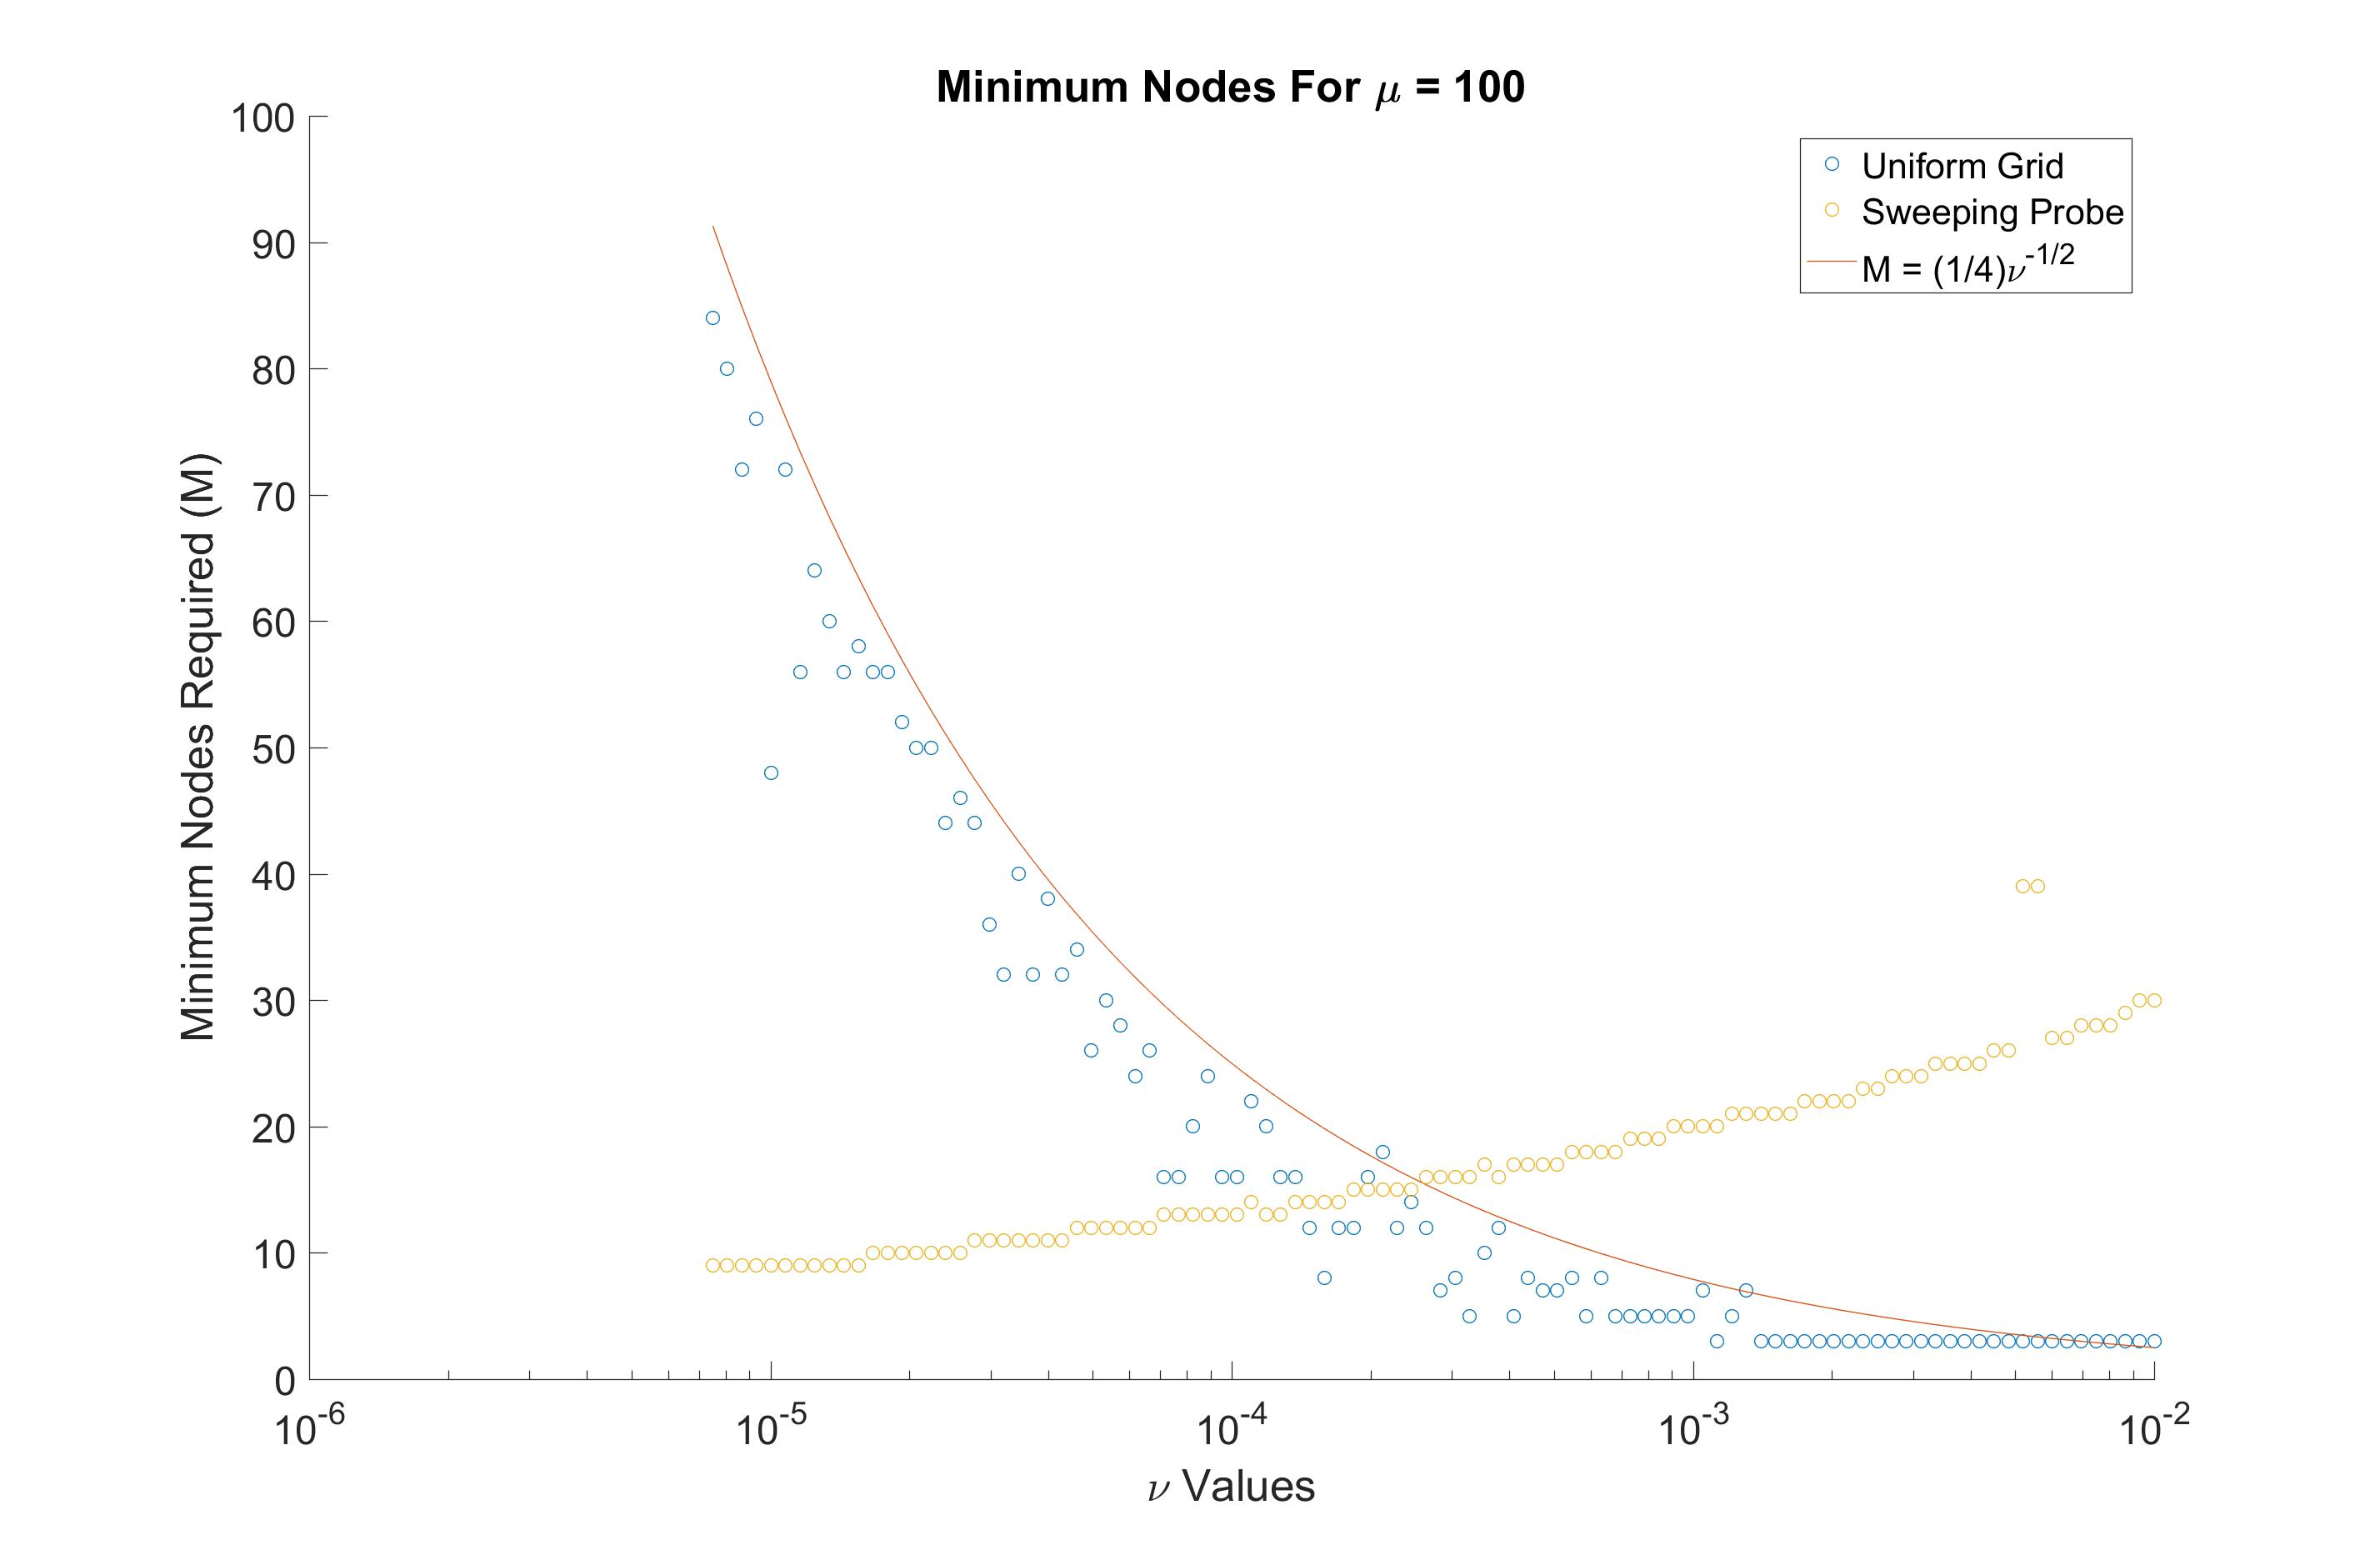
\includegraphics[scale=0.15]{Minimum}
	\caption{Minimum Nodes for Uniform Grid and Sweeping Probe required for convergence of 5e-15, $t=50$ units after ramp up period \\$\alpha = 1$ $N  =2^{12}$ $\mu = 100$ }
	\label{fig:min}
\end{figure}

\section{Concluding Remarks}
This study has established data assimilation as a viable alternative to the uniform grid.This requires far fewer points for convergence for certain $\nu$ values and doesn't require nodes to be placed in a special configuration. More work is required to determine the viability of this type of data assimilation in higher dimensions and its usability for other equations. 
\clearpage
% \section*{Acknowledgement}
% \noindent
% This research was partially supported by grant numbers... .
% 
 %~~~~~~~~~~~~~~~~~~~~~~~~~~~~~~~~~~~~~~~~~~~~~~~~~~~~~~~~~~~~~~~~~~~~
%\begin{scriptsize}
\bibliographystyle{amsplain}%amsalpha%amsplain%plain%abbrv
%\bibliographystyle{natbib}
\bibliography{thesis}
%\end{scriptsize}
%~~~~~~~~~~~~~~~~~~~~~~~~~~~~~~~~~~~~~~~~~~~~~~~~~~~~~~~~~~~~~~~~~~~~


%~~~~~~~~~~~~~~~~~~~~~~~~~~~~~~~~~~~~~~~~~~~~~~~~~~~~~~~~~~~~~~~~~~~~
\end{document}
%~~~~~~~~~~~~~~~~~~~~~~~~~~~~~~~~~~~~~~~~~~~~~~~~~~~~~~~~~~~~~~~~~~~~

